%---------------------------------------
%%% Figure histone modifications
\begin{figure}
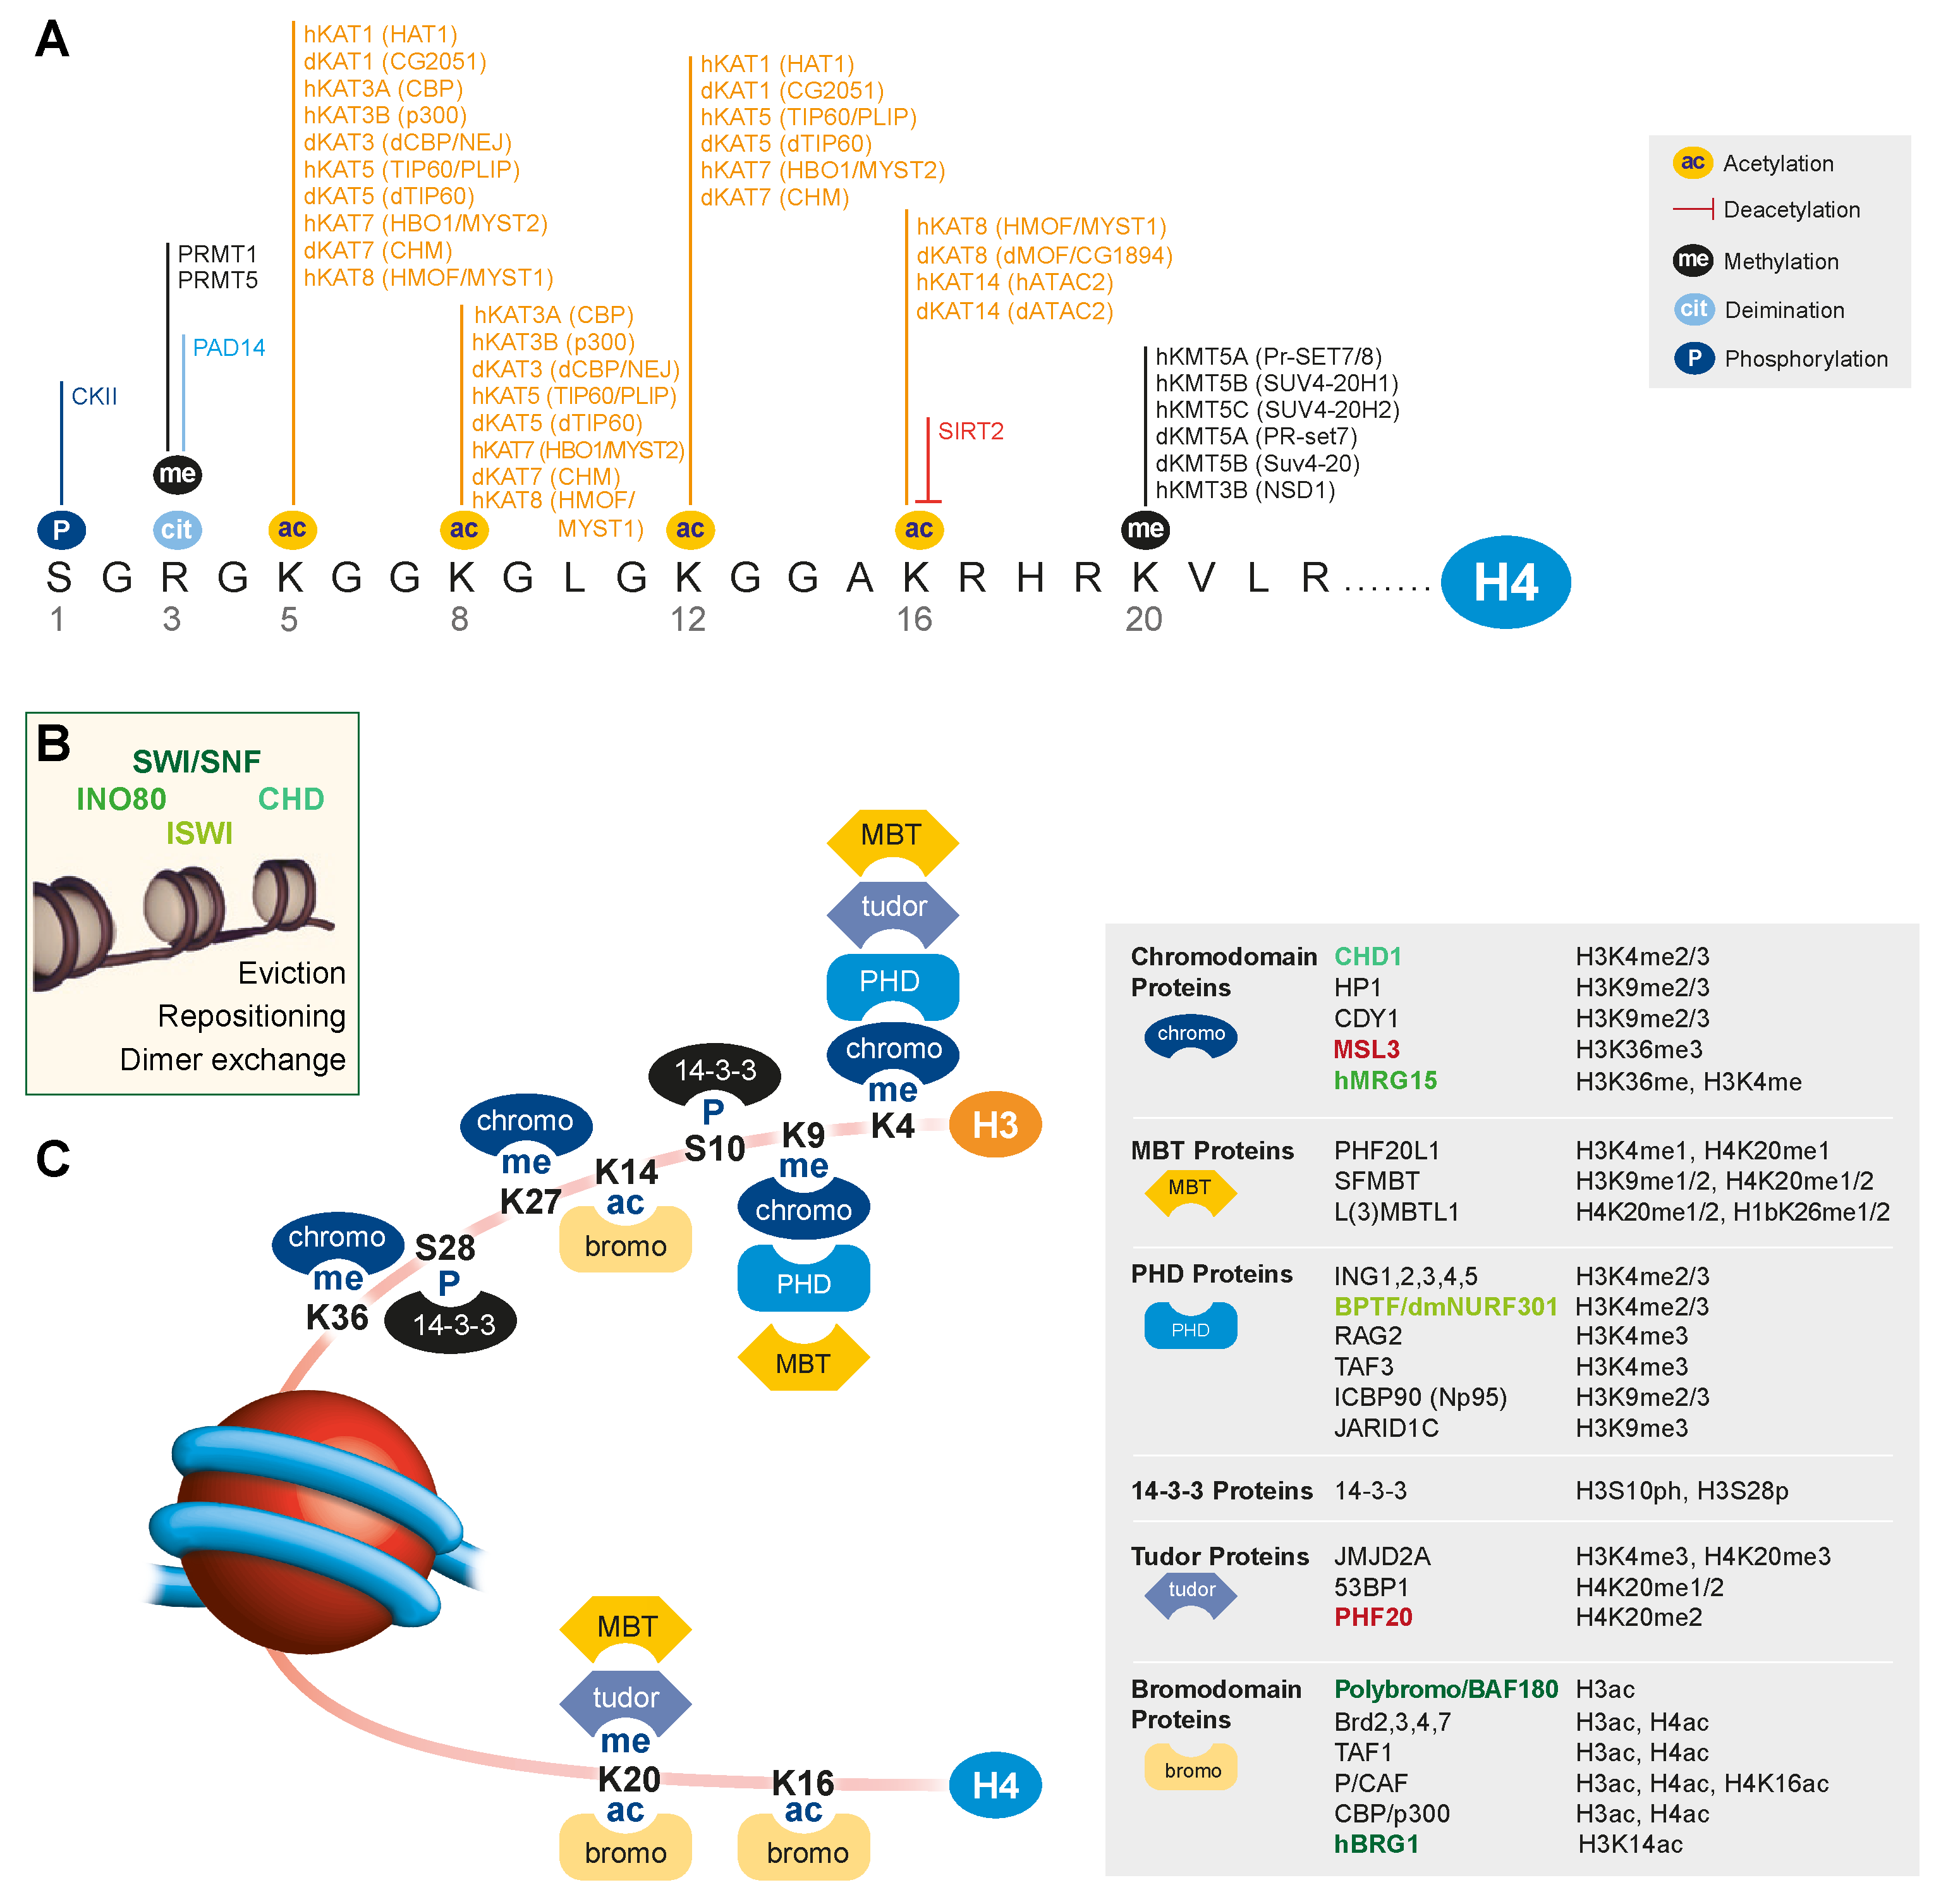
\includegraphics[width=1\textwidth]{Figures/histonesExtended.pdf}
\begin{footnotesize}
\caption[Exemplary histone modifications, their enzymes and histone-modification-recognizing protein domains.]{\textsf{Examples of histone modifications, corresponding enzymes and protein domains that recognize them.
\textbf{A)} Like for the other core histones, the tail of histone 4 (H4) contains numerous residues for covalent post-translational modifications of which some are shown here together with enzymes capable of catalyzing the respective mark in humans (h) and \textit{Drosophila} (d). Note that the different marks may have different biological meanings, e.g. methylation of H4K20 is associated with gene repression while acetylation of H4K16 is associated with gene activation (\fref{fig:histoneDistribution}). Moreover, the residues within the globular domains can also be modified (not shown). CKII = casein kinase II, PRMT = protein arginine methyltransferase, PAD2 = peptidyl arginine deiminiase, KAT = lysine acetyl transferase, KMT = lysine methyl transferase, SIRT2 = NAD-dependent deacetylase sirtuin-2. The image was taken from \citep{Abcam} and modified. See \tref{tab:HATs} for details on histone acetyl transferases.
\textbf{B)} Besides histone-modifying enzymes, chromatin remodellers greatly influence gene accessibility, too. There are four major families of ATP-dependent DNA translocases that can -- to varying degrees -- reposition, evict and replace nucleosomes. The INO80 family members are particularly important for DNA replication and repair as they can efficiently exchange histones while the multimeric complexes of the SWI/SNF family predominantly slide and evict nucleosomes \citep{Manelyte2013}.
\textbf{C)} Transcription factors (e.g. the transcription initiation factors TAF1 and 3), chromatin-remodelling complexes (shown in green, see B) and histone-modifying enzymes (e.g. the HATs CDY, p300 and P/CAF and the lysine demethylases JARID1C and JMJD2A) often contain domains that recognize specific histone modifications. Members of MOF-associated complexes are shown in red. The image was taken from \citep{Abcam} and modified.
}}
\label{fig:histonesExtended}
\end{footnotesize}
\end{figure}
%------------------------------------

